\textbf{System Architecture}

The \textbf{context diagram} of the system is shown in: Fig. \ref{fig:sys-context}, 
which indicates that the system has no dependences on outer systems.

\begin{figure*}[!ht]
	\centering
	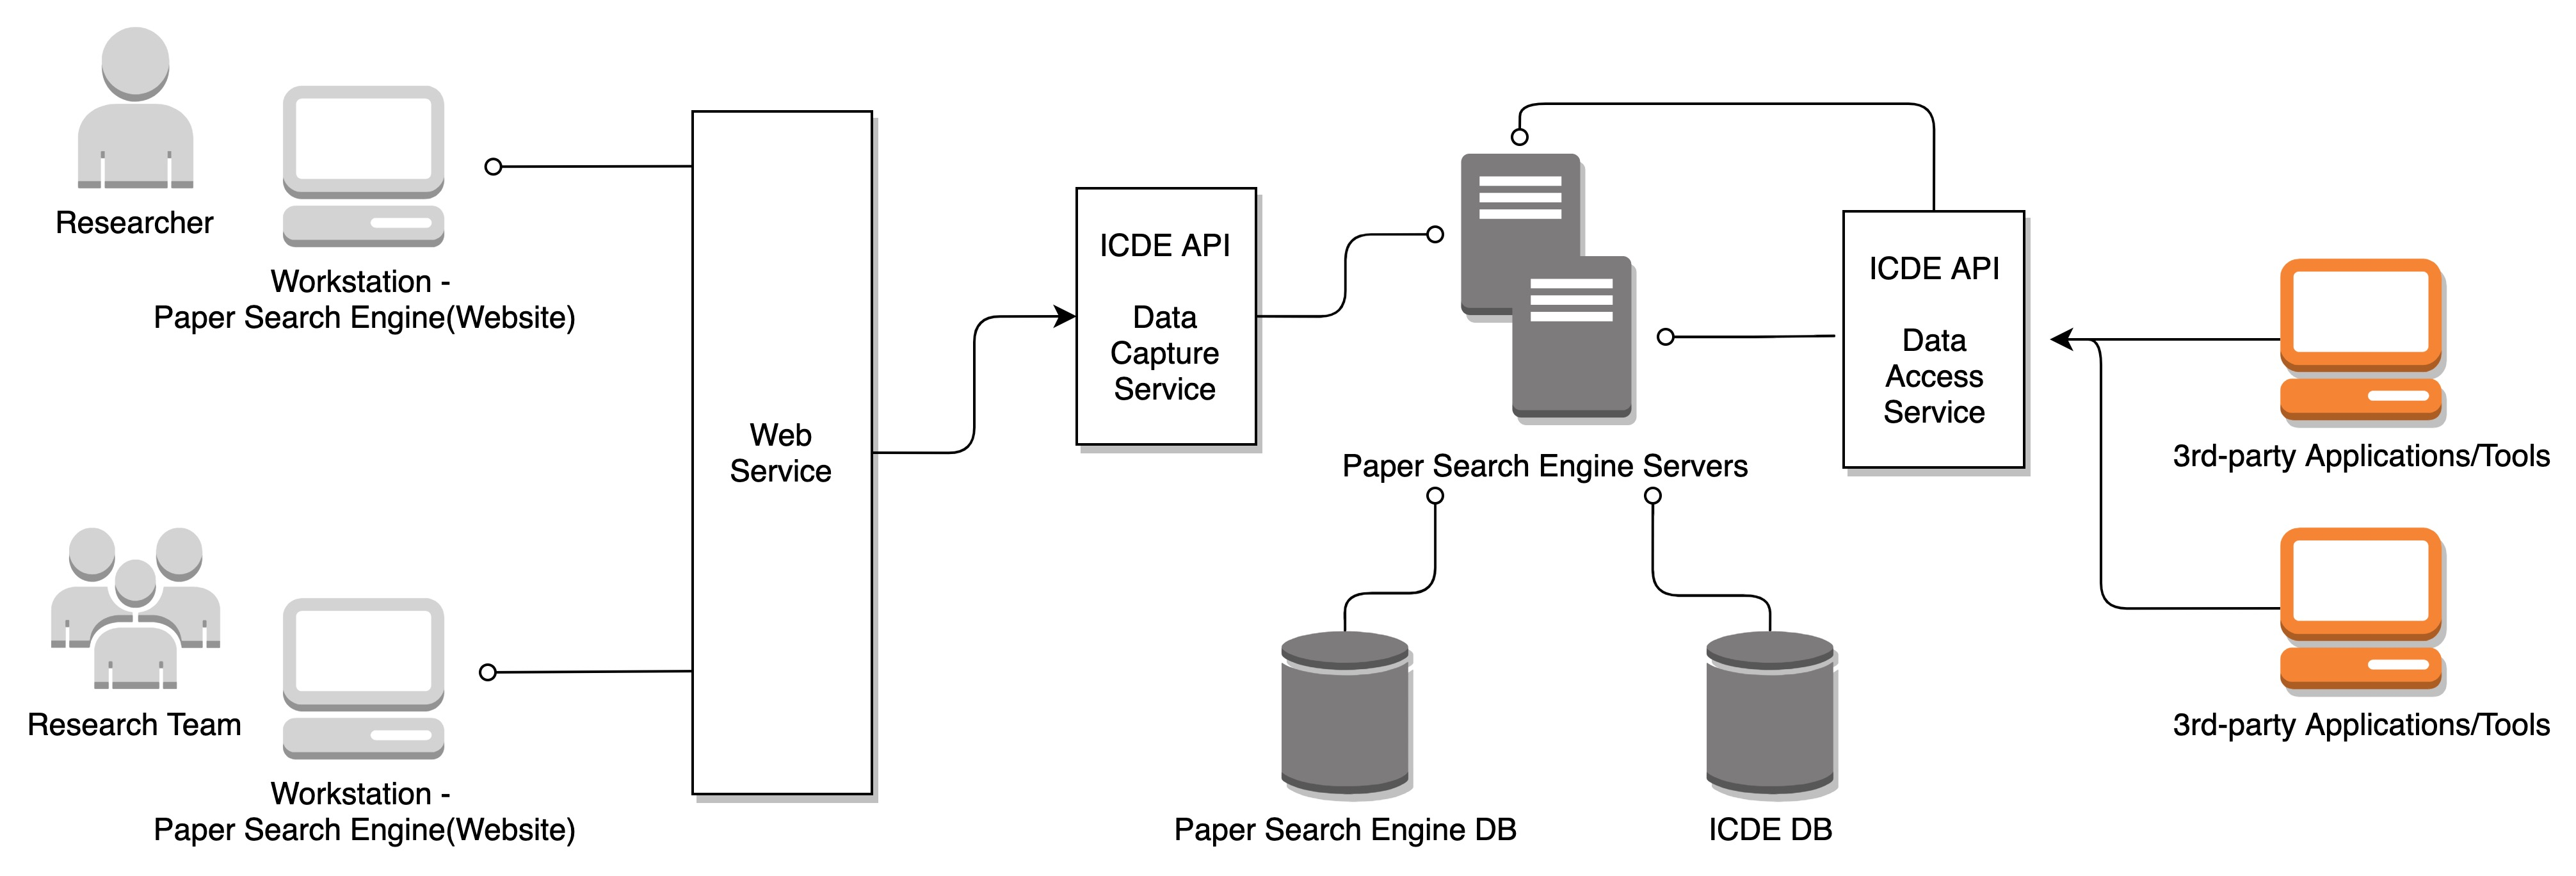
\includegraphics[width=0.8\textwidth]{./img/sys-context.png}
	\caption{System Context}
	\label{fig:sys-context}
\end{figure*}

The \textbf{system architecture diagram} is shown in: Fig. \ref{fig:sys-arch}.

The system will follow the MVC architecture since the client end of the system will be web browser. 
And obviously, it follows the layer pattern.

Notice that component with red box is designed for future development of this system itself. It might not be implemented within the scope of the class project but it will still have interfaces defined.

\begin{figure*}[!ht]
	\centering
	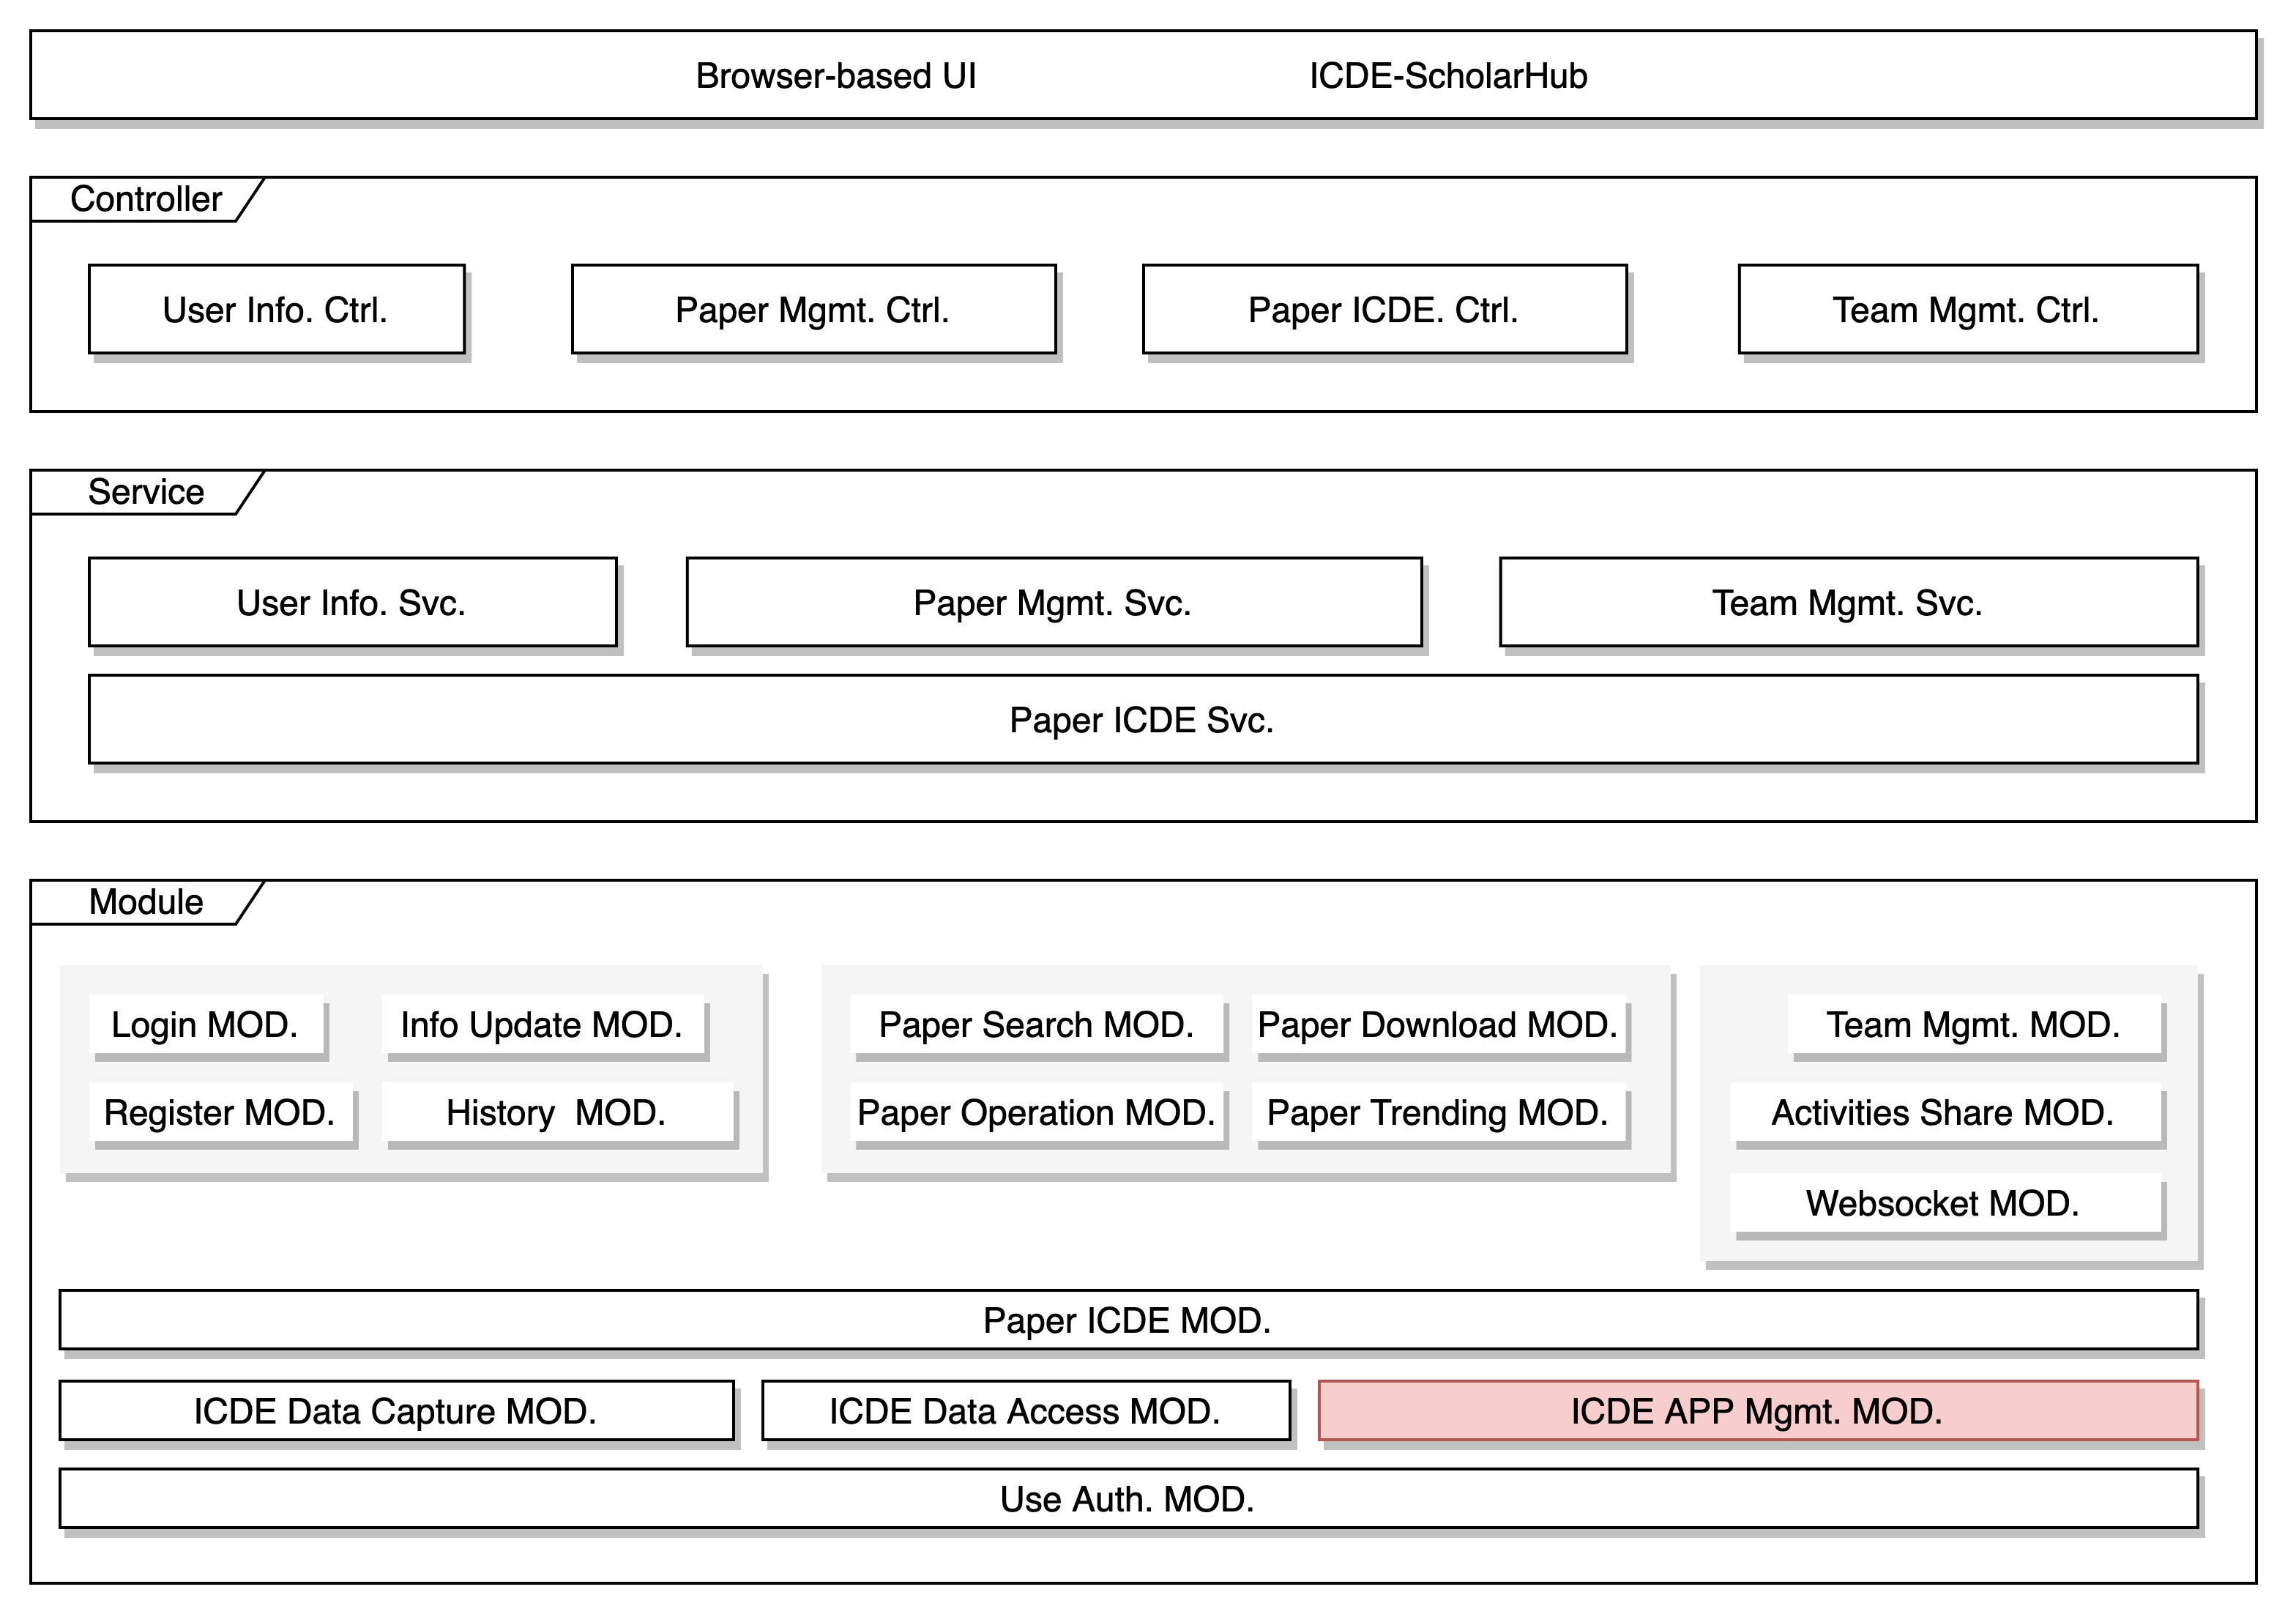
\includegraphics[width=0.8\textwidth]{./img/sys-arch.jpg}
	\caption{System Architecture}
	\label{fig:sys-arch}
\end{figure*}